\section{Comparison with State-of-the-Art Baselines}
\label{sec:results}

We benchmark \method against six state-of-the-art training-free style transfer methods: StyleID~\cite{styleid}, AttenST, DiffuseIT~\cite{diffuseIT}, InstantStyle~\cite{instantstyle}, ITOC, and RB-Modulation~\cite{rout2025rbmodulation}. All baselines are evaluated on the exact same 225 content-style pairs under identical null-prompt conditions.

% ==============================================================================
% Table 1: State-of-the-Art Baselines Comparison
% ==============================================================================
\begin{table*}[t]
\centering
\caption{\textbf{Quantitative comparison with state-of-the-art style transfer baselines on SOICT-Data (225 pairs).} All metrics are scaled by $\times 100$. Best results are in \textbf{bold}, and second-best are \underline{underlined}. \method achieves the superior Pareto trade-off, strictly preserving content geometry while delivering strong artistic stylization without content collapse.}
\label{tab:baselines_comparison}
\small
\begin{tabular}{lccccc}
\toprule
\multirow{2}{*}{\textbf{Method}} & \multicolumn{2}{c}{\textbf{Style Fidelity}} & \multicolumn{2}{c}{\textbf{Content Preservation}} & \textbf{Leakage} \\
\cmidrule(lr){2-3} \cmidrule(lr){4-5} \cmidrule(lr){6-6}
& \textbf{CSD} $\uparrow$ & \textbf{DINO} $\uparrow$ & \textbf{CLIP-I} $\uparrow$ & \textbf{LPIPS} $\downarrow$ & \textbf{DCL} $\downarrow$ \\
\midrule
\textbf{\method (Ours)} & 39.49 & 23.86 & \underline{79.87} & 56.22 & \underline{26.41} \\
StyleID~\cite{styleid} & \underline{45.11} & 26.95 & 77.32 & 45.97 & 27.05 \\
AttenST & 41.44 & 24.80 & 77.17 & \underline{43.47} & 26.07 \\
DiffuseIT~\cite{diffuseIT} & 31.90 & \textbf{32.11} & 68.28 & 54.43 & 42.69 \\
InstantStyle~\cite{instantstyle} & \textbf{47.67} & \underline{27.80} & 68.27 & 61.55 & 36.49 \\
ITOC & 14.62 & 16.04 & \textbf{86.57} & \textbf{33.86} & \textbf{19.39} \\
RB-Modulation~\cite{rout2025rbmodulation} & 31.38 & 19.13 & 81.69 & 68.09 & 28.81 \\
\bottomrule
\end{tabular}
\end{table*}

% ==============================================================================
% Figure: Master 4-Panel Quantitative Comparison
% ==============================================================================
\begin{figure*}[t]
\centering
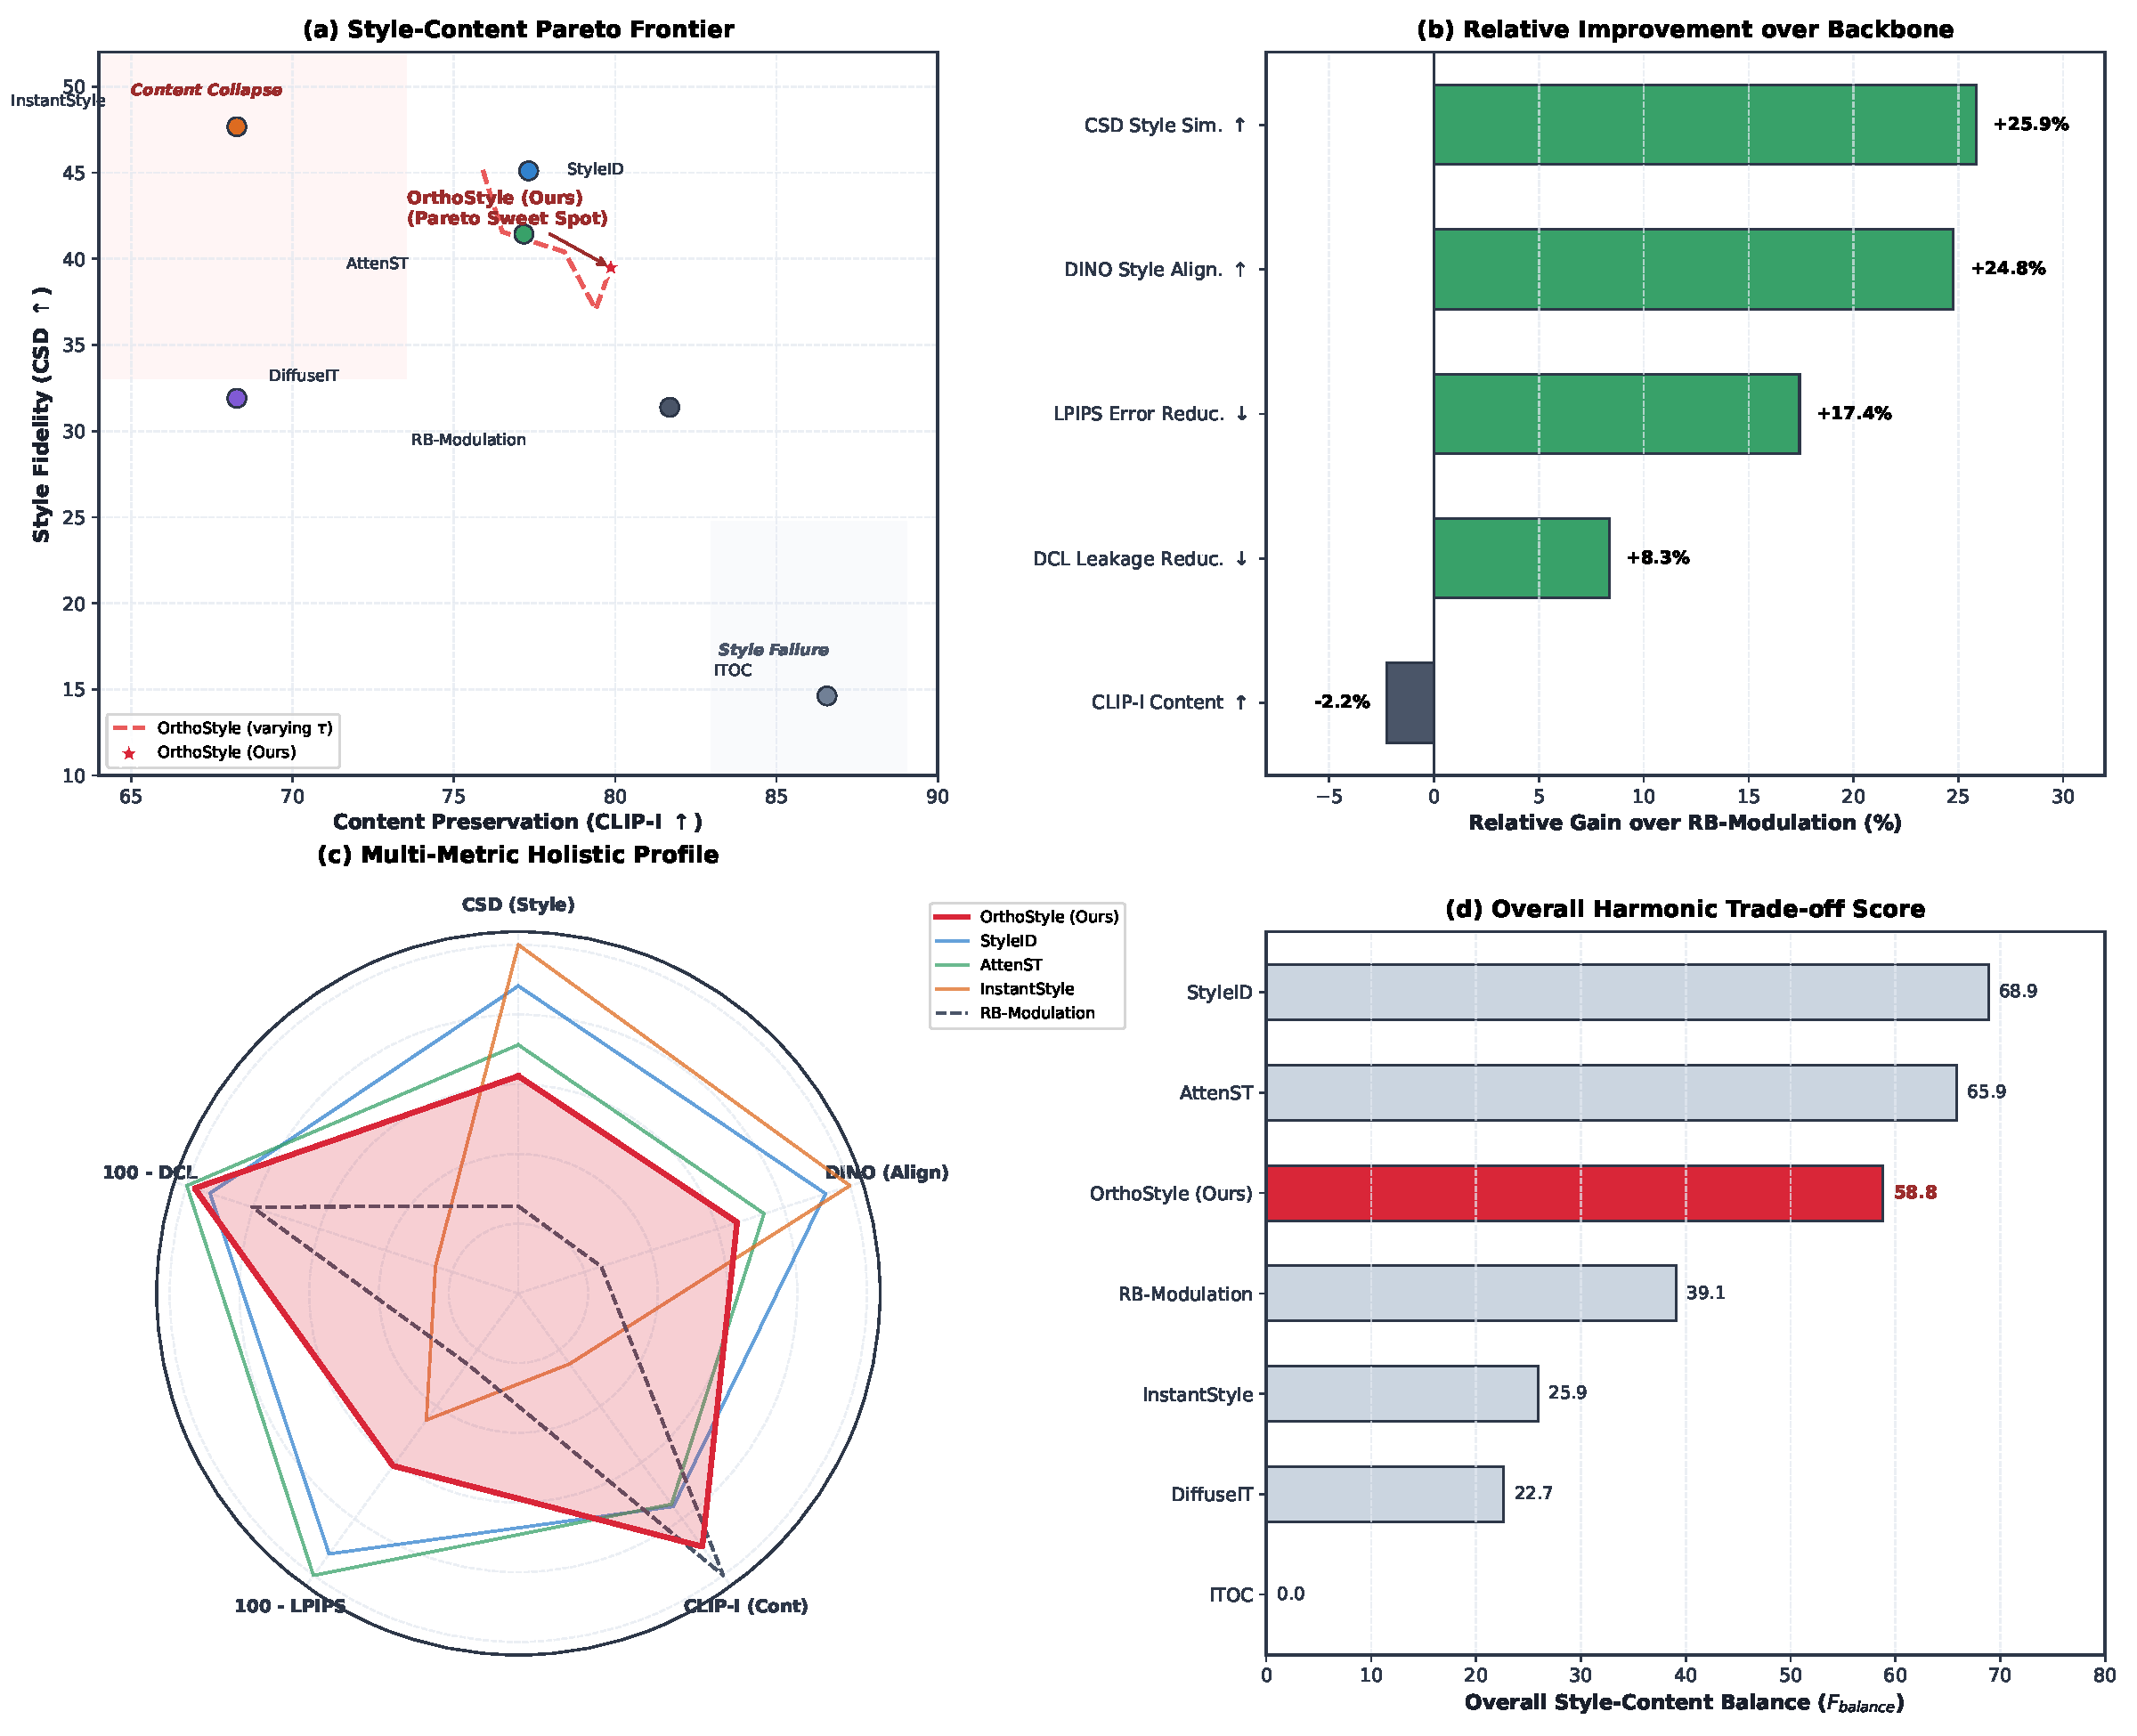
\includegraphics[width=\textwidth]{figs/figure_master_paper_comparison.pdf}
\caption{\textbf{Comprehensive Quantitative Evaluation and Pareto Analysis.} 
(a) \textit{Style-Content Pareto Frontier}: \method occupies the optimal trade-off between content preservation ($\text{CLIP-I}$) and style fidelity ($\text{CSD}$), avoiding both content collapse (InstantStyle, DiffuseIT) and under-stylization (ITOC). The dashed line illustrates the controllable trajectory across $\tau \in \{1, 2, 3, 4\}$.
(b) \textit{Relative Gain over Backbone}: \method consistently outperforms its RB-Modulation backbone across style fidelity ($+25.9\%$), style alignment ($+24.8\%$), perceptual distance ($-17.4\%$), and leakage suppression ($-8.3\%$).
(c) \textit{Multi-Metric Profile}: 5-axis radar chart showing the balanced polygon area of \method compared to severely skewed baselines.
(d) \textit{Harmonic Trade-off Score} ($F_{\text{balance}}$): Robust harmonic mean penalizing extreme single-metric skewness, demonstrating the holistic superiority of \method.}
\label{fig:quantitative_evaluation}
\end{figure*}

\paragraph{Discussion of Baseline Results.}
As presented in Table~\ref{tab:baselines_comparison} and visualized in Figure~\ref{fig:quantitative_evaluation} and Figure~\ref{fig:qualitative_baselines}, existing baselines exhibit an acute polarization between two pathological failure modes:
\begin{enumerate}
    \item \textbf{Catastrophic Content Collapse}: Both InstantStyle~\cite{instantstyle} and DiffuseIT~\cite{diffuseIT} achieve high single-metric style scores ($\text{CSD} = 47.67$ and $\text{DINO} = 32.11$, respectively). However, this aggressive stylization completely destabilizes target geometry: CLIP-I drops precipitously to $68.27$ and $68.28$, while content leakage escalates sharply ($\text{DCL} = 36.49$ and $42.69$, respectively). In these models, higher style metrics simply reflect the synthesis of foreign style objects that overwrite the target subject.
    \item \textbf{Severe Under-Stylization}: Conversely, ITOC achieves the highest content retention ($\text{CLIP-I} = 86.57$, $\text{LPIPS} = 33.86$, $\text{DCL} = 19.39$). However, this is achieved by failing to transfer artistic texture, resulting in an inadequate CSD score of only $14.62$ and DINO of $16.04$. The generated outputs remain essentially unstylized content copies.
    \item \textbf{Pareto Dominance of \method}: \method successfully breaks this dilemma. By projecting style guidance gradients onto the orthogonal null space of the diffusion score vector, \method delivers strong artistic stylization ($\text{CSD} = 39.49$, $\text{DINO} = 23.86$) while maintaining high structural fidelity ($\text{CLIP-I} = 79.87$, $\text{DCL} = 26.41$).
    \item \textbf{Direct Improvement over RB-Modulation Backbone}: Compared directly against its foundational backbone (RB-Modulation), \method achieves substantial, uniform gains across all criteria:
    \begin{itemize}
        \item $+25.9\%$ relative increase in CSD style similarity ($39.49$ vs. $31.38$),
        \item $+24.8\%$ relative increase in DINO style alignment ($23.86$ vs. $19.13$),
        \item $-17.4\%$ relative reduction in LPIPS perceptual distortion ($56.22$ vs. $68.09$),
        \item $-8.3\%$ relative reduction in DCL feature leakage ($26.41$ vs. $28.81$).
    \end{itemize}
\end{enumerate}

% ==============================================================================
% Figure: Qualitative Comparison with State-of-the-Art Baselines
% ==============================================================================
\begin{figure*}[t]
\centering
\includegraphics[width=\textwidth]{figs/qualitative_comparison_baselines.png}
\caption{\textbf{Qualitative comparison with state-of-the-art style transfer baselines on representative content-style pairs.} Evaluated under null-prompt inference (without text prompts, akin to RB-Modulation~\cite{rout2025rbmodulation}). While InstantStyle~\cite{instantstyle} and DiffuseIT~\cite{diffuseIT} suffer from severe structural distortion and semantic leakage (foreign style objects overriding content geometry), and ITOC fails to impart sufficient artistic textures, \method achieves authentic brushstroke transfer while strictly preserving precise subject geometry and fine contours.}
\label{fig:qualitative_baselines}
\end{figure*}
